\documentclass[10pt,a4paper,twoside]{article}
\usepackage[a4paper,top=20mm,bottom=20mm,outer=5cm]{geometry}
\usepackage[utf8]{inputenc}
\usepackage[english]{babel}
\usepackage{graphicx}
%\usepackage{hyperref}
\usepackage{amsmath}
%\usepackage{cleveref}
\usepackage{natbib}
\bibliographystyle{abbrvnat}
\setcitestyle{authoryear}

\title{Project Machine Learning\\--- Milestone 1 ---}

%%%%%%%%%%%%%%%%%%%%%%%%%%%%%%%%%%%%%%%
%                                     %
%   EVERYTHING BELOW CAN BE CHANGED   %
%                                     %
%%%%%%%%%%%%%%%%%%%%%%%%%%%%%%%%%%%%%%%

\author{Konstantin Ausborn, Timon Palm, Marco Rosinus Serrano}
\date{\today}

% our own packages
\usepackage{acronym}
\usepackage{wrapfig}
\usepackage{listings}
\usepackage{float}
\usepackage{hyperref}
\usepackage{cleveref}

% acronyms
\acrodef{ae}[AE]{Autoencoder}
\acrodef{vae}[VAE]{Variational Autoencoder}
\acrodef{vq}[VQ-VAE]{Vector Quantized Variatonal Autoencoder}
\acrodef{gan}[GAN]{Generative Adversarial Networks}
\acrodef{dnn}[DNN]{Deep Neural Networks}
\acrodef{bpp}{bits per pixel}
\acrodef{mse}[MSE]{Mean Squared Error}
\acrodef{psnr}[PSNR]{Peak Signal to Noise Ratio}
\acrodef{nll}[NLL]{Negative Log Likelihood}
\acrodef{fid}[FID]{Fréchet Inception Distance}
\acrodef{ssim}[SSIM]{Structural Similarity Index Measure}
\acrodef{ilsvrc}[ILSVRC]{ImageNet Large Scale Visual Recognition Challenge 2012}

\begin{document}
    \maketitle
    \section{Introduction}\label{sec:introduction}
    
Over the course of this machine learning project, we aim to implement a \ac{vq} as introduced by~\cite{vqvae} and to reproduce their results.
To begin, we focus solely on the field of 2D images, specifically using the ImageNet and CIFAR-10 datasets.
In the later stages of this project, we will have to decide to either go more in-depth, working on increasing the models capabilities in this one field, or widening our work over the other modalities touched upon by the paper introducing the model.

For the first milestone, we especially focus on the datasets and a baseline method for subsequent comparison to our final model.

This report is structured as follows: After a short intro into the \ac{vq}, we begin with an overview of the datasets we will use and the preprocessing and data-cleaning steps applied.
The next section describes the baseline method we implement, followed by a section on the evaluation metrics suitable for both these baselines and our future \ac{vq} model.
We close with a discussion of the results of our baseline models, questions we would like to solve over the course of the project and possible real world use-cases of the final model.


    \section{Datasets}\label{sec:datasets}
    Image generation forms an unsupervised learning task and therefore does not require labeled data.
The same applies for image compression.
Thus, any kind of image data can potentially be used for training and testing.

n the case of conditional image generation, labels can be of importance, though, as they might be used as a guiding
parameter in generation.
For instance, class labels or specific styles  can be used as an input to guide the generation towards a specific class or style.
In a later phase of this project we will use the class labels to guide the PixelCNN to generate instances of one specific class.

Generally speaking the image generation and reconstruction performance of a model is highly dependent on the quality
and diversity of the training data.

\subsection{Feature Extraction}\label{subsec:feature-extraction}
In machine learning, a set of features is ``good'' if it allows the model to achieve a certain task
efficiently.
For traditional, non-deep models, that means that features should aim to be informative, meaning that
they should have some predictive value towards the final goal.
In simple regression settings, this is the case if the feature correlates with the true value.
Furthermore, it is helpful for features to be independent form each other, as dependent features could overemphasize
their importance due to the higher frequency~\cite{featengineer}.

The reasons listed above are due to the high sensitivity of traditional ML models to small perturbations in data,
which calls for efficient feature engineering~\cite{lecun2015deep}
\textbf{maybe explain in 2 sentences how such features were found}
In modern deep learning settings, this sensitivity has decreased significantly~\cite{lecun2015deep}, which we also
expect to apply to all of our models.

However, normalization remains essential because features with larger scales tend to have a greater influence on gradients and
the final output compared to those with smaller scales.
Furthermore, normalized and standardized features generally lead to better convergence behaviour~\cite{mueller}.

As \ac{vq} works directly on pixel values, further feature extraction methods are not necessary.
Image pixels are numerical values with a spatial correlation that \ac{vq} leverage.
Since \ac{vq} follows the Encoder-Decoder structure, learning a compressed representation of the input image in latent
space, the model itself can be seen as a feature extraction method.

\subsection{Overview}\label{subsec:dataset-overview}
In the paper, the \ac{vq} is trained on three image datasets: \textit{ImageNet}, \textit{CIFAR-10}
, and video frames from \textit{DeepMind Lab}.
As stated in Section~\ref{sec:introduction}, we will focus our training on the ImageNet and CIFAR-10
datasets for now.

Both are among the most common image datasets used in machine learning.
While they were originally designed for image classification and detection tasks, their utility extends beyond
these applications; by discarding the labels, they can also be leveraged for image generation tasks.
An overview of these two datasets is provided in Table~\ref{tab:datasets}

\begin{table}[ht]
    \begin{tabular}{lllll}
        Dataset  & \# train images & \# test images & \# classes & image size           \\ \hline \hline
        ILSVRC   & 1.281.167       & 100.000        & 1000       & 8x10px - 9331x6530px \\
        CIFAR-10 & 50.000          & 10.000         & 10         & 32x32px              \\ \hline \hline
    \end{tabular}
    \caption{Key data on ImageNet/\ac{ilsvrc}}
    \label{tab:datasets}
\end{table}

\subsection{ImageNet}\label{subsec:imagenet}

\begin{wrapfigure}{r}{0.4\textwidth}
    \centering
    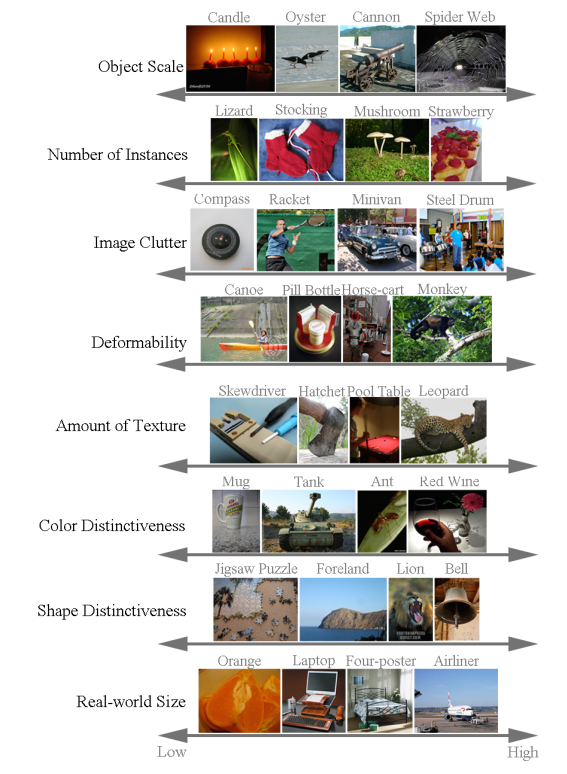
\includegraphics[width=0.4\textwidth]{../../sample_images/imnet_dimension}
    \caption{Eight diversity dimensions of the ImageNet dataset~\cite{imagenet_breakdown}}
    \label{fig:imnet_dimensions}
\end{wrapfigure}

The full ImageNet dataset consists of 14.197.122 hand-labeled photographs collected from flickr and other search
engines, distributed over 21841 \textit{synonym sets} from the
\textit{WordNet} hierarchy, pursuing to cover most nouns in the English language as described by~\cite{wordnet}.

When talking about ImageNet, many authors refer to the \ac{ilsvrc} dataset.
It is a subset of the full dataset, containing 1.281.167 unique labeled training images and 100.000 labeled test
images distributed over 1000 classes, with an additional 50.000 unlabeled validation images for benchmarking
purposes, which we will not consider.

Three key computer vision tasks are benchmarked by the \ac{ilsvrc} dataset: object classification, object
localization and object detection.
They address three fundamental computer vision questions: \textit{What is in the image?}, \textit{Where is it?} and
\textit{How many are there?}.
For \ac{ilsvrc}, each image is annotated with a class id and bounding boxes of objects.
The collected images neither contain missing values nor duplicates and every image belongs to exactly one class.

All information on ImageNet and ILSVRC described up until this point is taken from~\cite{imagenet_breakdown}, which
evaluates the history of \ac{ilsvrc} in its first five years.
Hereinafter, we will refer to this subset as ImageNet if not stated otherwise.

The dataset aims to replicate the distribution of natural photographs, specifically including a diverse range of
examples across the eight dimensions illustrated in Figure~\ref{fig:imnet_dimensions}.
Thereby, models trained on it can generalize along these.



\textbf{Class Balance}
To not introduce bias, the dataset should be sufficiently balanced between the classes.

In the ImageNet dataset, a majority of classes contain 1300 examples, with some classes having fewer examples, as
shown in Figure~\ref{fig:imnet_dist}.

Based on this, we assess the class distribution in the ImageNet dataset as sufficiently balanced.
Most classes contain an equal amount of samples, and the classes with fewer examples are still represented by a
reasonable number of images.
All of them contain more than half the maximum number of samples.
Moreover, the three outlier classes with the lowest sample numbers are classes referring to specific dog
breeds with 732, 738 and 754 samples, respectively.
The general class of dogs is therefore still well represented.

\begin{figure}[ht]
    \centering
    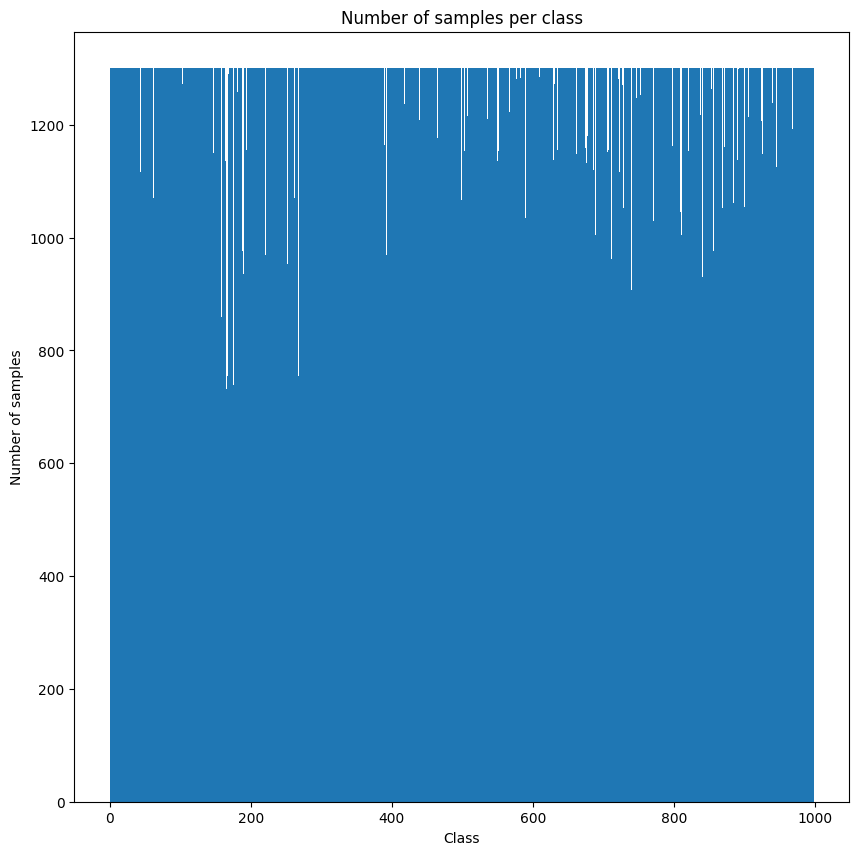
\includegraphics[width=0.5\textwidth]{../../sample_images/imagenet_dist}
    \caption{Distribution of images per class in the ImageNet dataset}
    \label{fig:imnet_dist}
\end{figure}

\textbf{Image Shapes}
Upon examining, we found that the images have highly irregular resolutions.
The width and height ranges from 8-9331px and 20-6530px, respectively, with a mean resolution of 471.7x404.7 pixels.
Figure~\ref{fig:imnet_sizes_err} depicts the resolution ranges for each class.

As to be seen in figure~\ref{fig:optimum_resolution}, some images have a very irregular ratio, which imposes a challenge
for resizing.
Very small images do not contain enough information, which when upscaled, result in a blurry image (illustrated in
figure~\ref{fig:small_image}).

\subsubsection{Data Cleaning and Preprocessing}
In order to train the \ac{vq} on the ImageNet dataset, we will do the following preprocessing steps.

\begin{itemize}
    \item \textbf{Data Cleaning}
    Based on our knowledge from examining the image shapes, remove images with a resolution below 32px on any axis
    \item \textbf{Image Resizing}
    For training and testing, we resize all images to 128x128 pixels, similar to the paper.
    We use a composition of random cropping to extract a square image and resizing it to 128x128 pixels with
    the \texttt{v2.RandomResizedCrop} function from the TorchVision package.
    We set \texttt{scale=(0.2, 1.0)} and \texttt{ratio=1} to crop a square image with a sufficient area in
    relation to the original image, and enable anti-alias to reduce artifacts.
    \item \textbf{MinMax Normalizing and Standardization}
    Due to the observations on normalization and standardization described in Subsection
    ~\ref{subsec:feature-extraction}, we scale each channel from integers in $\{0,\dots,255\}$ to floats on
    $[0,1]$.
    We also standardize the images with the mean $\mu = (0.485, 0.456, 0.406)$ and standard deviation
    $\sigma = (0.229, 0.224, 0.225)$ of ImageNet for the three color channels, respectively.
\end{itemize}

Example images from ImageNet dataset after preprocessing are depicted in figure~\ref{fig:imnet_example_normalized}.

\subsection{CIFAR-10}\label{subsec:cifar-10}
CIFAR-10~\cite{cifar10} is another popular image classification dataset, as well as the larger version CIFAR-100.
CIFAR-10 consists of 60.000 32x32 pixel images, which are distributed over 10 classes.
The dataset is split into 50.000 training images and 10.000 test images.
The classes are mutually exclusive, so each image belongs to exactly one class.
The classes are: \textit{airplane, automobile, bird, cat, deer, dog, frog, horse, ship, truck}

The train set contains exactly 5000 images per class, while the test set contains 1000 images per class.
No image belongs to more than one class and there are no missing values or duplicates in the dataset.

\subsubsection{Preprocessing}
As the images in the CIFAR-10 dataset are already 32x32 pixels, we do not need to resize them.
Hence, we will only apply MinMax Normalizing and potentially Standardizing, same as for the ImageNet data.

Example images from the CIFAR-10 dataset are shown in figure~\ref{fig:cifar10_example_normalized}.

    \section{Evaluation Metrics}\label{sec:evaluation-metrics}
    \subsection{Compression}\label{subsec:compression}
For compression, the most straightforward metric is to measure the reduction of memory required to
store the data.
To normalize over image resolution, we choose to evaluate the \ac{bpp}.

The second, and less objective measure, is image similarity after reconstruction.
While the \ac{mse} and by transfer \ac{psnr} describe pixel-wise similarity very well, it is not
always optimal to judge perceived similarity for humans, as can be seen in Figure~\ref{fig:mse_ssim}.

\begin{figure}[ht]
    \centering
    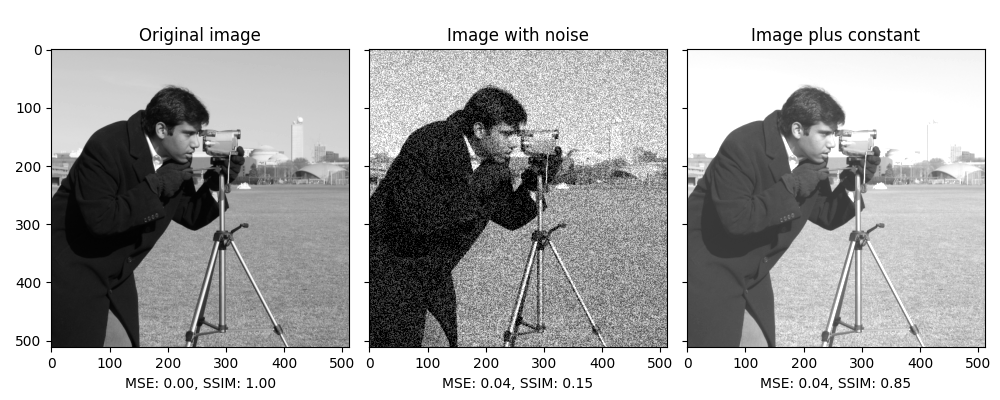
\includegraphics[width=0.8\textwidth]{images/ssim_mse}
    \caption{from~\cite{scikit-ssim}}
    \label{fig:mse_ssim}
\end{figure}

To overcome these limitations we will use the \ac{ssim}, a metric working under the assumption that human visual
perception is highly adapted for extracting structural information from a scene, that has been

Even though this analysis favours \ac{ssim}, we use \ac{mse} as our loss function for our baseline models,
since the \ac{vq} implementation we plan to replicate does the same, and we want to maximize comparability.
We use \ac{ssim} for result evaluation, and add \ac{psnr} values for further work later on.

\subsection{Image Generation}\label{subsec:image-generation}
An important metric in Image Generation and the one used to argue about the strong performance of the \ac{vq} in the
paper is the \ac{nll} normalized to the amount of pixels (dimensions) in an image, given in bits/dim.
A lower number indicates a higher likelihood of generating the test data given our model.
The bits/dim number is rooted in information theory, and describes the average number of bits required to
compress the test data with the entropy coding scheme that is optimal for a model~\cite{shannon}.

The \ac{fid}, introduced by~\cite{fid}, is another interesting metric.
It compares the distribution of features of a generator with that of real images via a network trained on a big
dataset, often also imagenet.

Another criterion not to be left out is the classic human turing test, as in evaluating the images by hand.
Even though this is not scalable, it is the ultimate classifier for human perception, and can be a good starting
point.

As on metrics we found, but decided not to use: The paper that introduced \ac{fid} it also shows that it is more
consistent than a previous, similar metric, the inception score, which we will therefore leave out.
Another sometimes utilized evaluation metric that research has shown to better avoid are Parzen Windows Estimates~
\cite{note_on_eval}.

Overall, since we have not yet implemented any Image Generation functionality, it remains to be seen which of these
criteria are of which worth to us.

TODO: INTRODUCE FORMULAS FOR THE CRITERIONS

\subsection{Class differences}


    \section{Baseline method and evaluation}\label{sec:baseline-method-and-evaluation}
    In order to judge different performance measures of our final model, we require a baseline.
Such a baseline needs to align to the collection of tasks described in Section~\ref{sec:introduction} as close as
possible to allow for good comparability of results.

\subsection{Non-ML Baseline: JPEG}\label{subsec:jpeg}
While much of the current work in realistic high resolution image generation, e.g. \ac{gan} or \ac{vq}, is based on
\ac{dnn}, the field of image compression is well researched both in-, and outside deep architectures~\cite{compression}.
Non-ML approaches are still dominant on the web as can be seen in Figure~\ref{fig:file_formats}.
Due to this prevalence of such approaches, we compare our results to the popular JPEG format for lossy compression.

\begin{figure}[H]
    \centering
    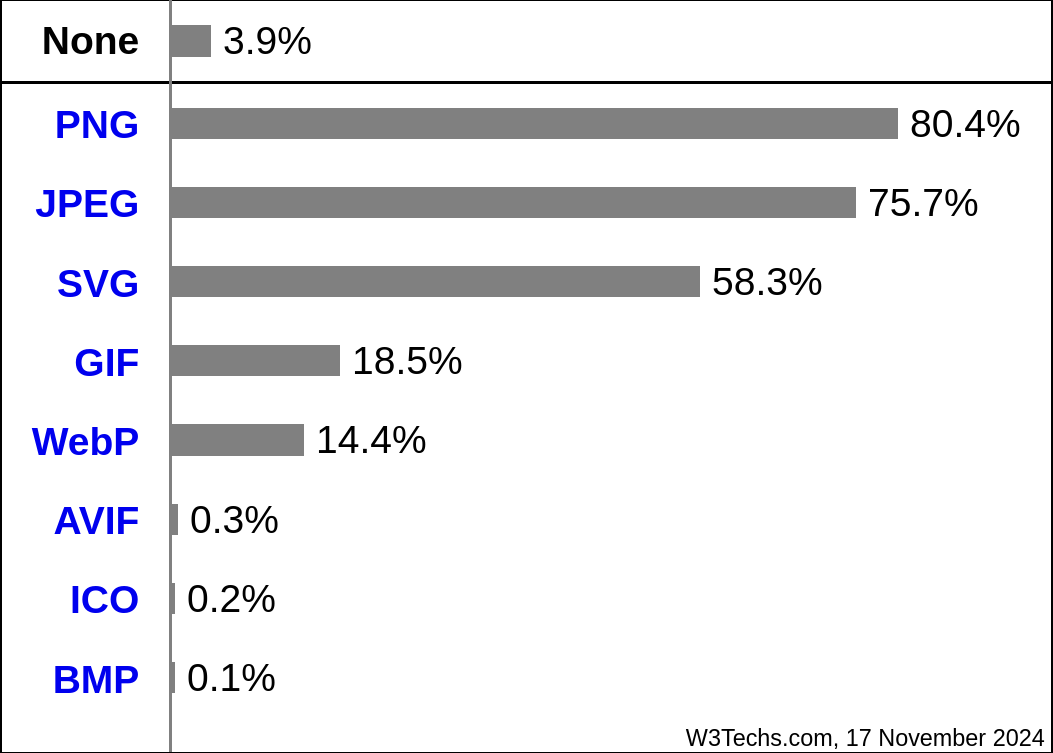
\includegraphics[width=0.3\textwidth]{images/formats}
    \caption{Percentages of websites using various image file formats~\cite{img_file_format}}
    \label{fig:file_formats}
\end{figure}

There exist multiple machine learning approaches with a setup similar to that of the \ac{vq}
i.e.\ generative models with latent representations such as \ac{gan}.
Differences in architectural details make these hard to compare against each other.
Revisiting the example of \ac{gan} as described by~\cite{gan}, the latents, like those in the \ac{vq} after
training the PixelCNN, approximate a distribution similar to the training data.
However, a key difference is that these latents cannot be obtained by encoding real-world data, making it impossible to
directly compare the compression task.

\subsection{Autoencoder}\label{subsec:autoencoder}
We selected a basic \ac{ae} as our general baseline method because it serves as the foundation for the original
\ac{vae}, which was later developed into the \ac{vq}.

A basic \ac{ae}, as described by~\cite{autoenc} and shown in Figure~\ref{fig:ae}, is a neural network designed to compress and reconstruct data. In our case, the input is an image. During the encoding stage, the network compresses the input data to a lower-dimensional representation using one or more fully connected hidden layers.
The output of this stage is passed to a latent layer, whose dimensionality determines the size of the compressed representation.

The decoding stage, which mirrors the structure of the encoding stage, upsamples the latent representation to reconstruct the original input.
The final output, known as the reconstruction, has the same shape as the input data, allowing for a direct comparison between the two.

The model can be trained by applying gradient descent on some form of cost function that describes reconstruction error
like \ac{mse}, theoretically pushing the network to encode the information most important to deconstruction in the
latent.

The similarities to \ac{vq} enable highly comparable results, as the \ac{ae} can be adjusted to closely match the
size, training requirements, and inference costs of the \ac{vq}.
In implementing the \ac{ae} baseline, we follow the same architecture as the \ac{vq} wherever feasible.
Specifically, we replace the fully connected layers of the standard \ac{ae} with the downsampling layers and
residual blocks from the \ac{vq} implementation in our reference paper.
This modification is expected to significantly enhance performance, as convolutional \ac{ae}s have been shown to
outperform basic feed-forward \ac{ae}s in image reconstruction tasks, as demonstrated by~\cite{convae}.

\begin{figure}[H]
    \centering
    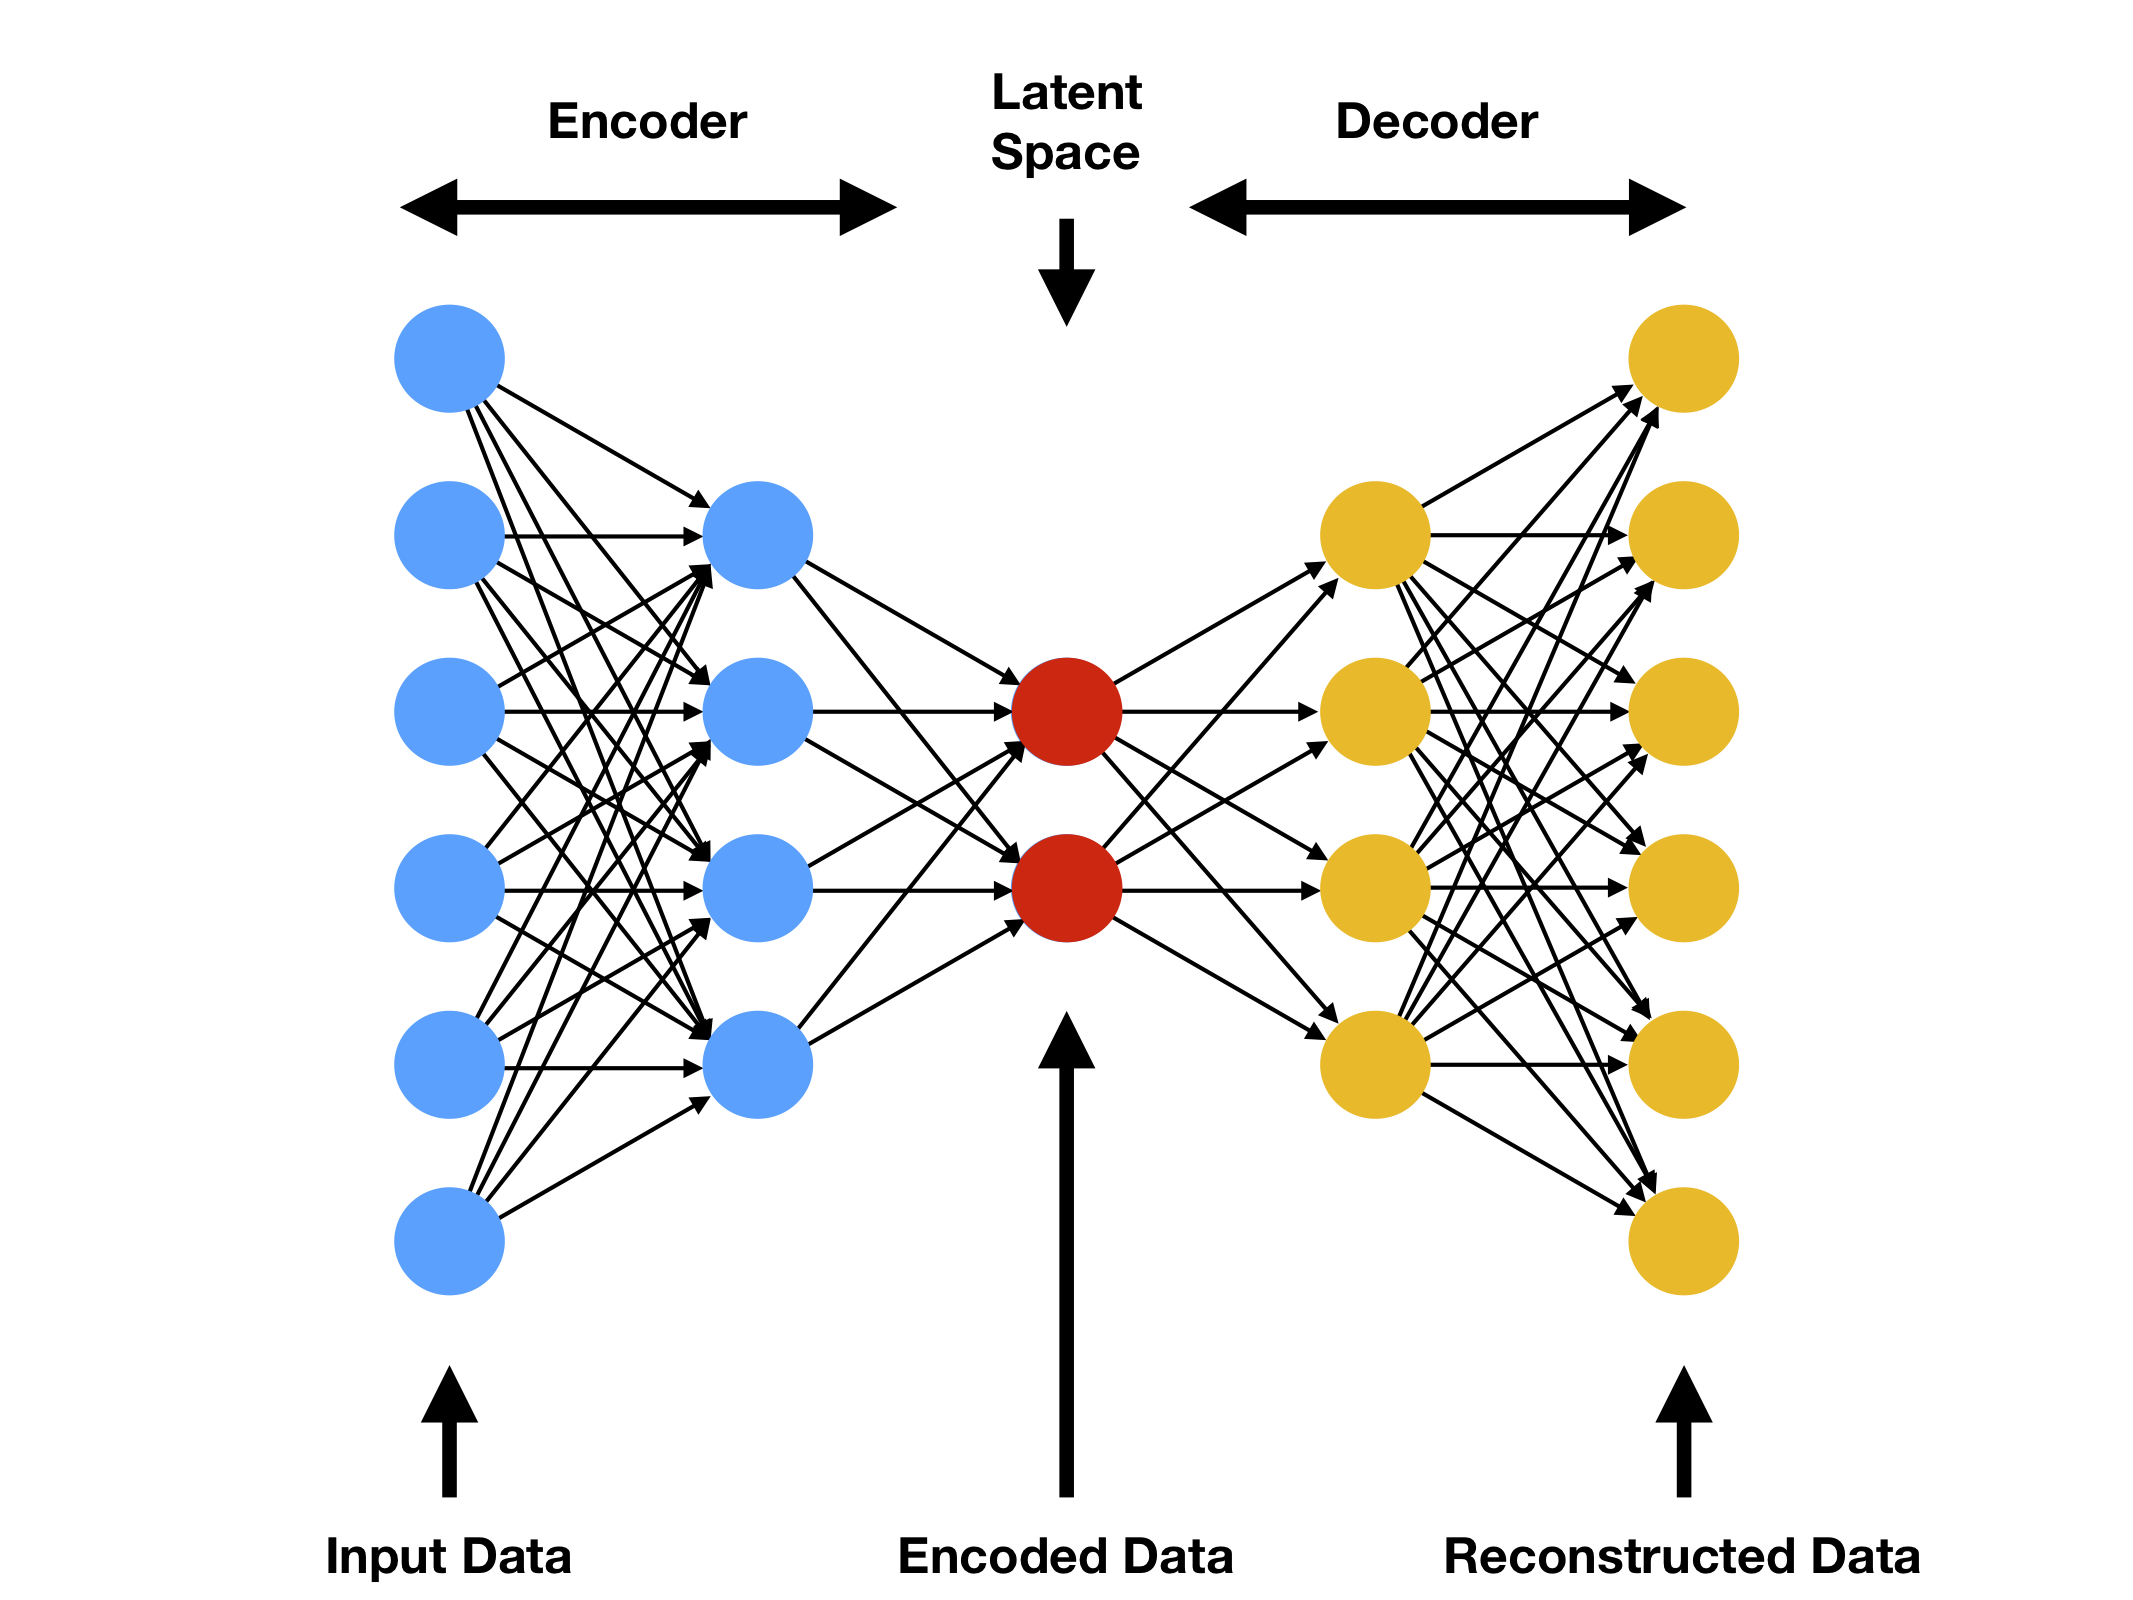
\includegraphics[width=0.5\textwidth]{images/ae}
    \caption{Illustration of a basic \ac{ae} architecture from~\cite{ae_pic}}
    \label{fig:ae}
\end{figure}

\subsection{Variational AE}\label{subsec:variational-ae}
Examining the differences between the different evolutionary steps towards the \ac{vq} could prove to be valuable
for our understanding of its performance.
Therefore, we also implement a \ac{vae}, which substantially differs from the \ac{ae} in the way that latents are
generated.
When constructing the neural network, we follow the same paradigm as with the \ac{ae} before, using the same
encoding and decoding layers as far as possible.
The important difference of the VAE is that its encoder outputs a random variable
$\boldsymbol{\hat{z}} \sim \mathcal{N}(\boldsymbol{\mu_\theta}, \text{diag}
(\boldsymbol{\sigma_\theta}))$. $\boldsymbol{\hat{z}}$ is obtained using the
reparameterization trick, which consists in sampling $\boldsymbol{z}
\sim \mathcal{N}(0, I)$ and then computing $\boldsymbol{\hat{z}} =
\boldsymbol{\mu_\theta} + \boldsymbol{z} \odot \boldsymbol{\sigma_\theta}$.
$\boldsymbol{\mu_\theta}$ and $\boldsymbol{\sigma_\theta}$ are deterministic
outputs of the last convolutional layer of the \ac{vae} encoder.
This allows to optimize the model using the ELBO loss which in turn enables us to not only
reconstruct the input, but to learn a posterior distribution $p(x|z)$ while
the encoder $q(z|x)$ tries to be as close as possible to $p(z)$.
Thus enabling us to generate new dataset samples by sampling $z \sim p(z)$ and then feeding
it through the decoder.
    \section{Discussion}\label{sec:discussion}
    The following sections will discuss the results of our baseline experiments, further ideas for the project, and real-world applications of the project.

\subsection{Baseline Experiments}\label{subsec:baseline-results}
    We present some results of our baseline training runs. We did an examplarily training for 10 epochs on a subset of ImageNet to see that it converges. The subset contained 100.000 images with 1000 samples per class. See ... for the full configuration details.

    \subsubsection{Autoencoder}\label{subsubsec:autoencoder}
        We were able to show that our implementation of an \ac{ae} is able to reconstruct images from the ImageNet dataset. W

        For this trainig, we used a latent dimension of 32x32x2 pixels, which means 4 bits per pixel for an 128x128x3 input images. That is a compression rate of 4,7 \% compared to the original image size.

        We are surprised by the results of our basic \ac{ae} and its capability to reconstruct images. Even with a realitively small latent dimension and only 10 epochs of training it is able to reconstruct images with a satifiying human percetiple quality.
        

\subsubsection{Class Differences}\label{subsubsec:class-differences}

\subsection{Real World Use of the Datasets}\label{subsec:real-world-applications}
\ac{cifar} and ImageNet have been foundational datasets for over a decade and a half.
Over time, their primary use-case has shifted from being cutting-edge datasets for training state-of-the-art models
to serving as a base for experiments and benchmarks.

The prominent role of ImageNet in its early days is evident when looking at AlexNet~\cite{AlexNet}.
The groundbreaking paper on training a \ac{cnn} on ImageNet using GPUs has been cited an extraordinary 166 thousand
times as of the time of this report and is regarded as one of the pivotal moments in the rise of \ac{dnn}.

Today, the most recent text-to-image generation models rely on much larger datasets, often containing billions of samples.
A notable example is LAION-5B, as described by~\cite{laion5b}, which is utilized in models such as Stable
Diffusion, based on the work of~\cite{stable_diff}.
However, upon closer examination of this paper, the ongoing significance of ImageNet becomes evident.
It can be observed that it is used as a dataset for training experimental networks, where using larger, modern
datasets would be prohibitively expensive.
Additionally, metrics such as the \ac{fid}, discussed in Section~\ref{sec:evaluation-metrics}, are calculated using
ImageNet, further highlighting its continued importance in research.

Similar trends can be observed for CIFAR-10.
However, its low resolution limits its applicability for benchmarking modern approaches to image generation.

Based on these observations, while we expect our final model to produce some believable results, we do not anticipate
achieving the level of visual fidelity demonstrated by state-of-the-art image generation models.

\subsection{Dataset}
    As the results of our exemplary training runs of only a small subset of training data show, our models already exhibit promising results. We are confident that with the full ImageNet dataset, we will be able to train our models to a better perfomance, at least in terms of reconstruction.

    Sampling functionality has not yet been implemented; however, we are certain that the dataset is equally suitable for training generative models. The dataset will likely not be a limitation for our task.

    The biggest challenge but also the biggest advantage of the ImageNet dataset is its size. The size imposes a challenge in terms of assessing the data, i.e. the shapes, properties of indivisual classes and their distribution. It is impossable to look at all the images, so we had to draw conclusions from sample image inspection and statistical analysis.

    On the other hand, the size and diversity of the data is a huge advantage for training the models. The models will be able to learn a wide range of features and patterns, and to generalize it to unseen data.


\subsection{A prospect on further Experiements}\label{subsec:further-ideas}
    We utilize the structural similarity index as a metric for image similarity to evaluate the reconstruction quality of our models \ref{subsec:compression}. For comparison to the paper, we still use \ac{mse} loss for training our \ac{ae}. Though, as discussed in \ref{subsec:compression}, \ac{mse} might not be the optimal metric in terms of human perception.

    \ac{ssim} is a metric for precisely this purpose, so we think our models might benifit from using it as a loss function instead of \ac{mse}. In ~\cite{ssim_as_loss}, it is shown that using a loss function trageted to human perception can improve the quality of convolutional neural networks for image reconstruction, in particular using \ac{ssim}. 

\subsection{Working Title: Final words}\label{subsec:final-words}
    Image reconstrution as well as image generation are two realitively well researched topics. Presumably, because of their wide range of applications. While the most prominent methods, i.e. \ac{ae} and \ac{vae}, are two simple yet powerful models, they still have their limitations. 

    \ac{ae} are powerful reconstructors, but they are not able to generate new images, because of their deterministic nature and their discrete latent representation.

    \ac{vae} can sample in the latent space and generate new images by virtue of their stochastic properties. Yet, you sometime favour a discrete latent over latent distributions, because of their simplicity, interpretability and compatibilty with other modalities ~\cite{vqvae}.

    \ac{vq} is an attempt to fill that gap. It enables to reconstruct images, generate new samples while having a discrete latent representation.

\vskip 1em
\textbf{A Note on Overfitting:}
Overfitting refers to the phenomenon where a model starts to memorize the training data instead of learning useful
features, in turn not generalizing well to unseen data.

While theoretically, this may very well be an issue with \ac{ae} and \ac{vae}, we have not experienced this happening
yet with either when training with adequate training-set sizes.
This is likely due to the large dataset sizes we use and the inductive bias of the convolution operation~
\cite{citationNeeded}.
    \bibliography{bibliography}
    \section{Appendix}\label{sec:appendix}
    \begin{figure}[H]
    \centering
    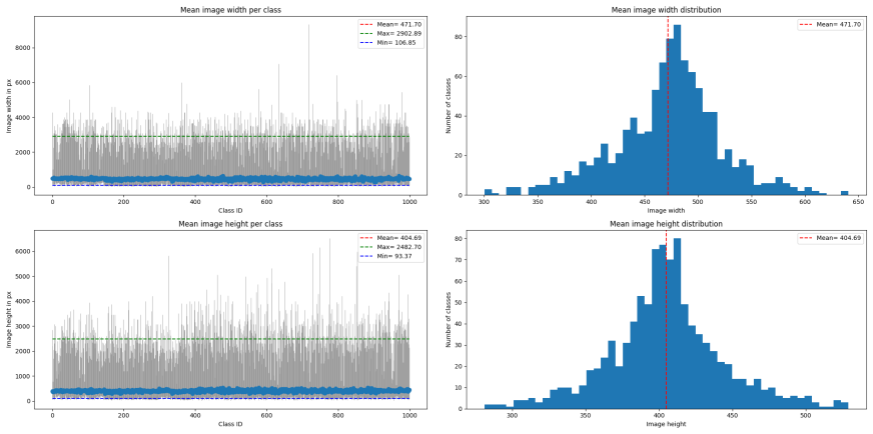
\includegraphics[width=\textwidth]{images/imagenet_histo_errorbars}
    \caption{Left: Image resolution deviations in the ImageNet dataset across classes,
        Right: Histogram of image resolutions in the ImageNet dataset}
    \label{fig:bigboy}
\end{figure}

\begin{figure}[H]
    \centering
    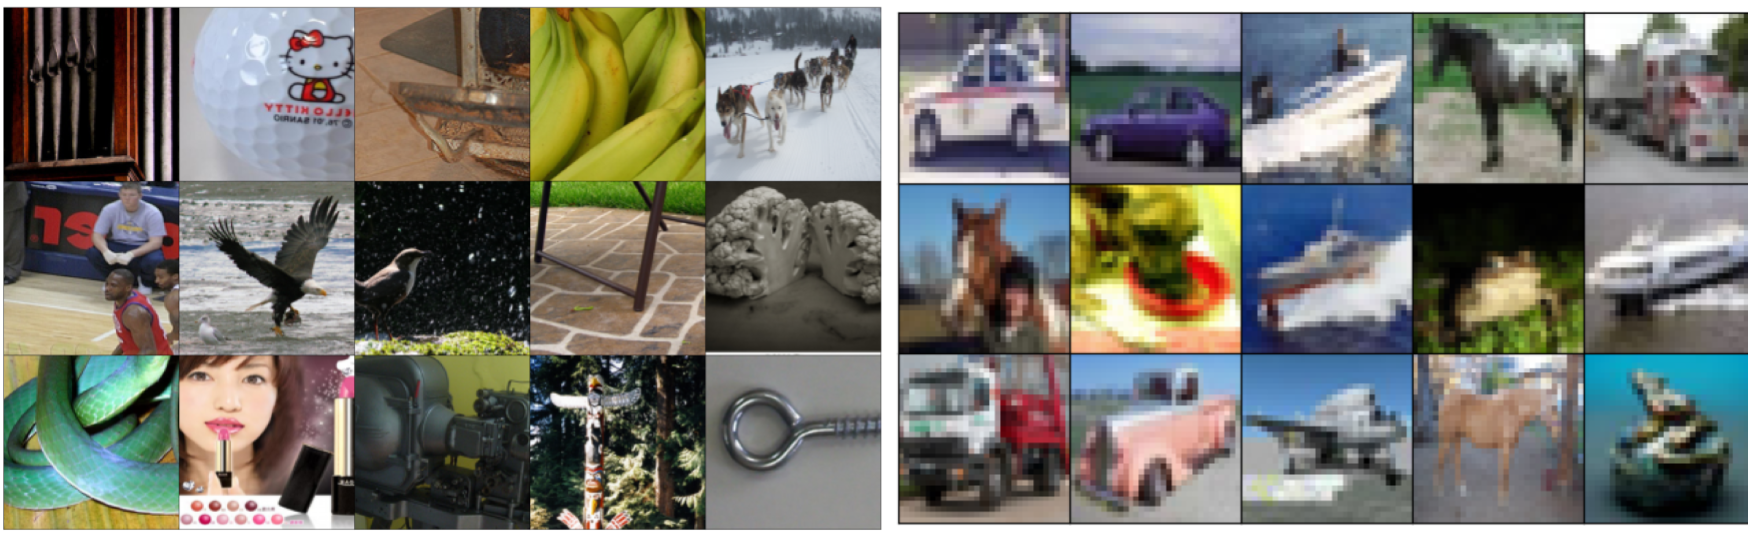
\includegraphics[width=\textwidth]{images/normalized_images_cifar_imagenet}
    \caption{Left: Example images from the ImageNet dataset randomly cropped and resized to 128x128 pixels and standardized, Right: Example images from the CIFAR-10 dataset standardized}
    \label{fig:cifar_imagenet_normalized}
\end{figure}

\begin{figure}[H]
    \centering
    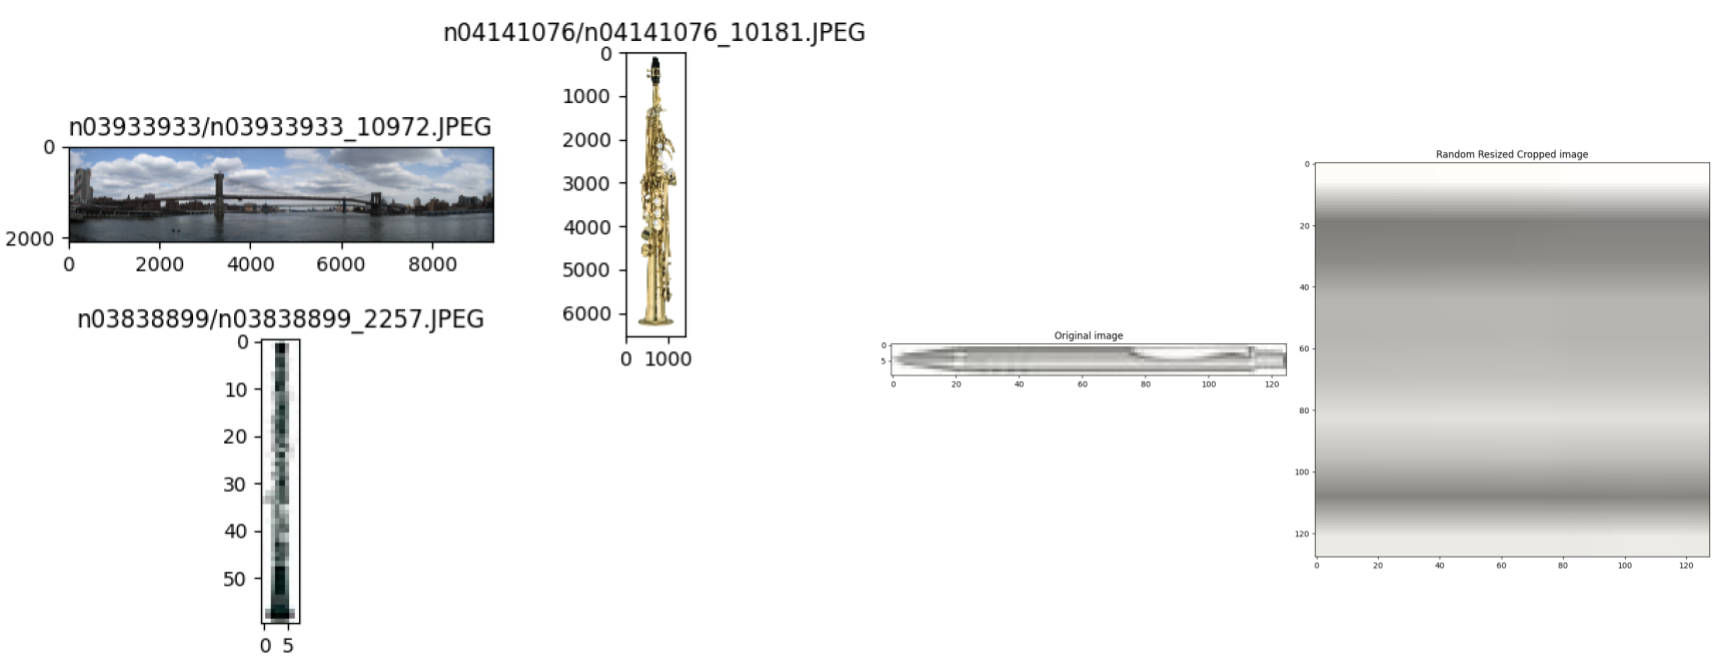
\includegraphics[width=0.7\textwidth]{images/extreme_shapes}
    \caption{Example images from the ImageNet dataset with very unregular resolution ratios}
    \label{fig:optimum_resolution}
\end{figure}
\end{document}
